%\document{article}
\documentclass[UTF8]{ctexart}
\usepackage{amsmath}
\usepackage{graphicx}
\usepackage{fancyhdr}
\usepackage{float}
\title{银行模拟}
\author{朱河勤   PB16030899}
\pagestyle{fancy}

%\chead{银行模拟}
\lfoot{朱河勤   PB16030899}
\rfoot{2017/10/21}
\begin{document}
\maketitle
\tableofcontents
\section{需求分析}
\paragraph{1}
创建银行排队窗口,还可以增加vip通道,可通过队列来实现,队列可以用链表封装得到
\paragraph{2}
每个客户可以存款,取款,如果银行钱不够,让客户处于等待状态,直到银行的钱足够
\paragraph{3}
如果排队的队伍过长,在最后的可以选择较短的队伍
\paragraph{4}
把所有事件打印出来
\section{概要设计}
\subsection{链表}
ADT linkList\{\\
\paragraph{数据对象}:D=\{$a_i| a_i , i =0,1 2,\dots,n$\}\\
\paragraph{数据关系}:R1 = \{$<a_{i-1},a_i> | a_{i-1},a_i in D ,i = 2,3,\dots,n$\}\\
\paragraph{基本操作}:
\subparagraph{s = linkList()}创建一个链表s
\subparagraph{s.append(x)} 向lst尾部增加节点x
\subparagraph{x = s[i]}将x引用链表第i个 节点
\subparagraph{del s[i]}删除链表第i个 节点
\subparagraph{s[i] = x}将链表第i个 节点赋值x
\subparagraph{s.insert(i,x)}将链表第i个 节点前插入x
\subsection{双端队列}
ADT linkList\{\\
\paragraph{数据对象}:D=\{$a_i| a_i , i =0,1 2,\dots,n$\}\\
\paragraph{数据关系}:R1 = \{$a_i,<a_{i-1}> | a_{i-1},a_i in D ,i = 2,3,\dots,n$\}\\
\paragraph{基本操作}:
\subparagraph{s = queue()}创建一个队列s
\subparagraph{s.append(x)} 向lst尾部增加节点x
\subparagraph{x = s[i]}将x引用第i个 节点
\subparagraph{s.pop()}右边第一个元素出队
\subparagraph{s.popleft()}左边第一个元素出队
\subparagraph{s.appendleft()}左边第一个元素进队
\}
\section{详细设计}
\subsection{用户类型}
\begin{figure}[H]
  \centering
  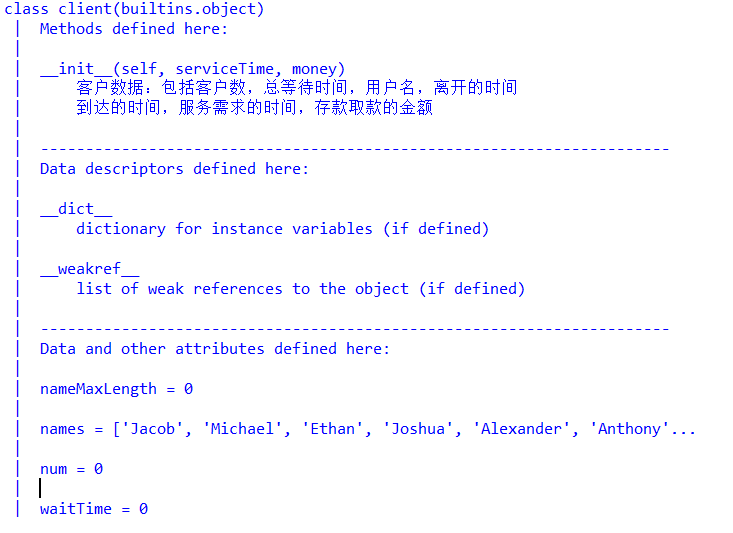
\includegraphics[width=1\textwidth]{client.png}
\end{figure}
\subsection{窗口类型}
\begin{figure}[H]
  \centering
  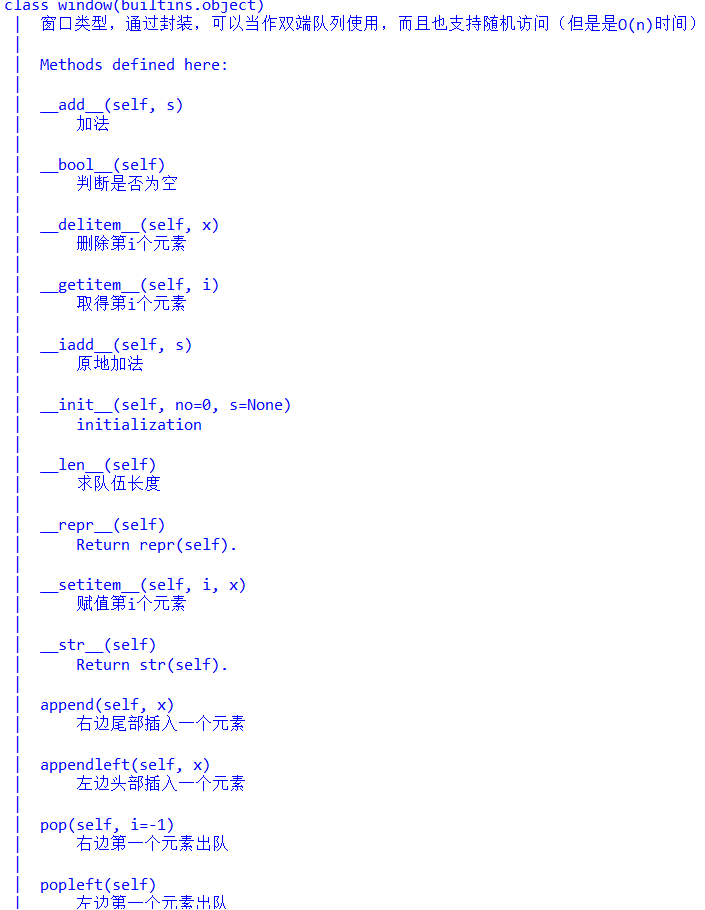
\includegraphics[width=1\textwidth]{window.png}
\end{figure}
\subsection{银行类型}
\begin{figure}[H]
  \centering
  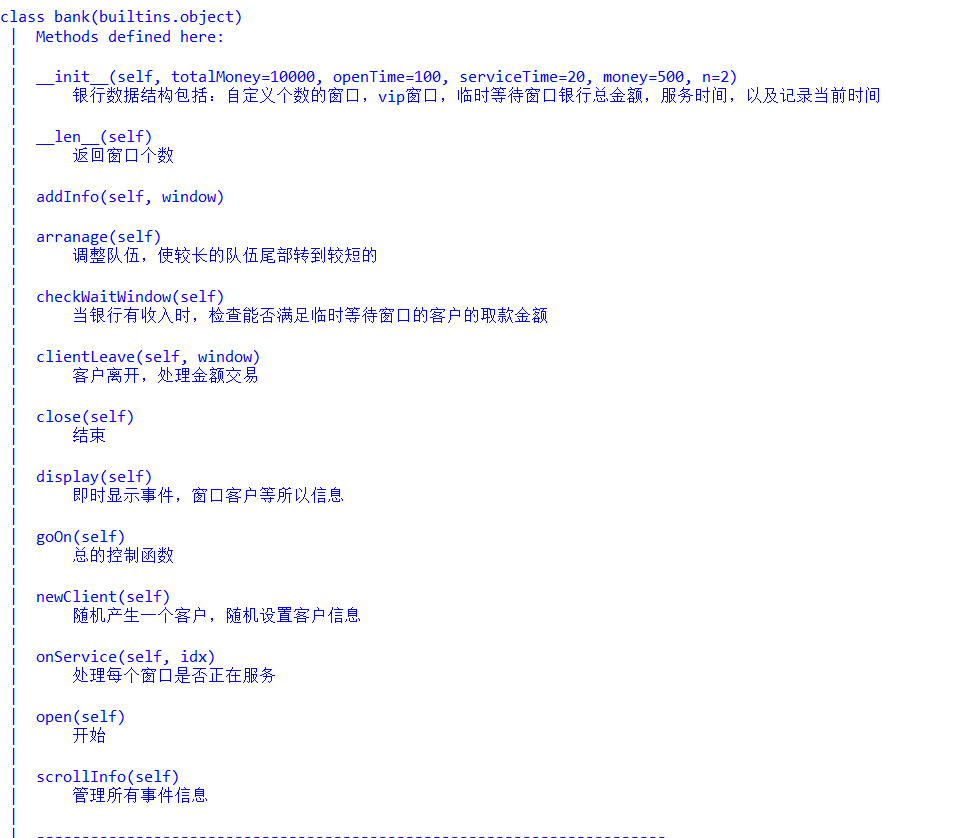
\includegraphics[width=1\textwidth]{bank.png}
\end{figure}
\subsection{显示信息的函数代码}
\begin{figure}[H]
  \centering
  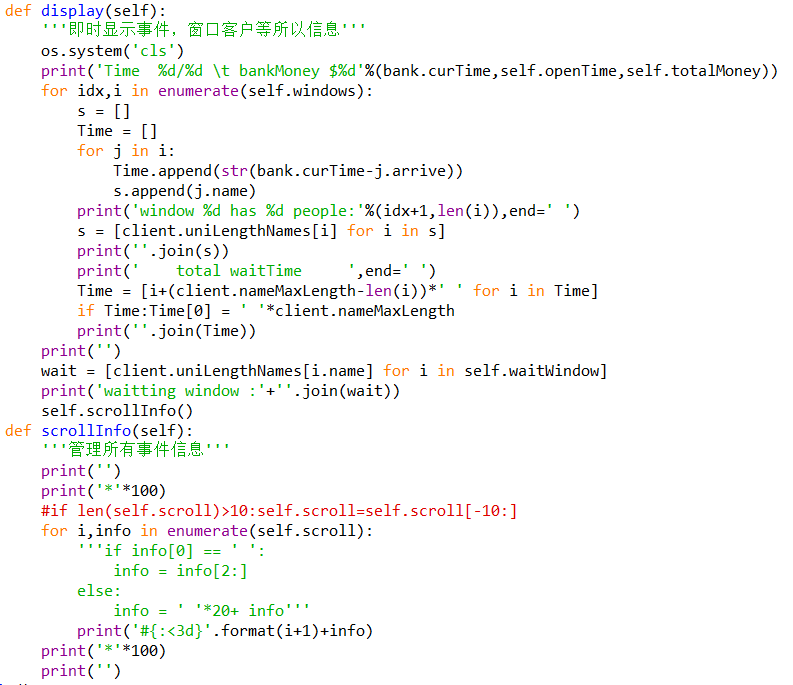
\includegraphics[width=1\textwidth]{display.png}
\end{figure}
\section{调试分析}
\paragraph{1}
整体上,定义了window,client,bank类型, 主要的操作在bank类中的方法实现
\paragraph{2}
为了标识每个用户,我给每个用户设置了一个英文名(可以有重复)。我在网上搜索了最常用的100个英文名,然后赋值到python交互模式,以字符串保存,然后用正则表达式匹配英文名
\paragraph{3}
在输出信息上,我通过清屏来更新信息。为了对齐更加美观,为另存了一个字典来保存每个客户统一长度的名字
\section{用户手册}
本程序需要在安装了python下的环境运行,可以在python的ide中使用文件运行,也可以通过命令行运行python bankSimaulate.py\\
下面为程序运行界面
\begin{figure}[H]
  \centering
  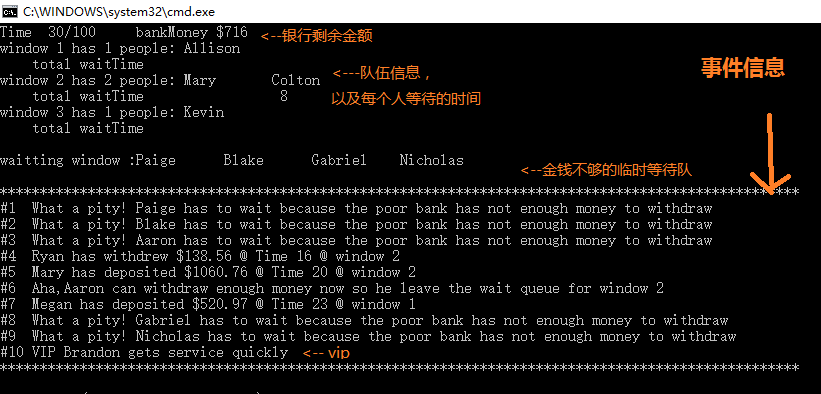
\includegraphics[width=1\textwidth]{demonstrate.png}
\end{figure}
\section{测试结果}
\subsection{输入10000,100,20,50,2}
\begin{figure}[H]
  \centering
  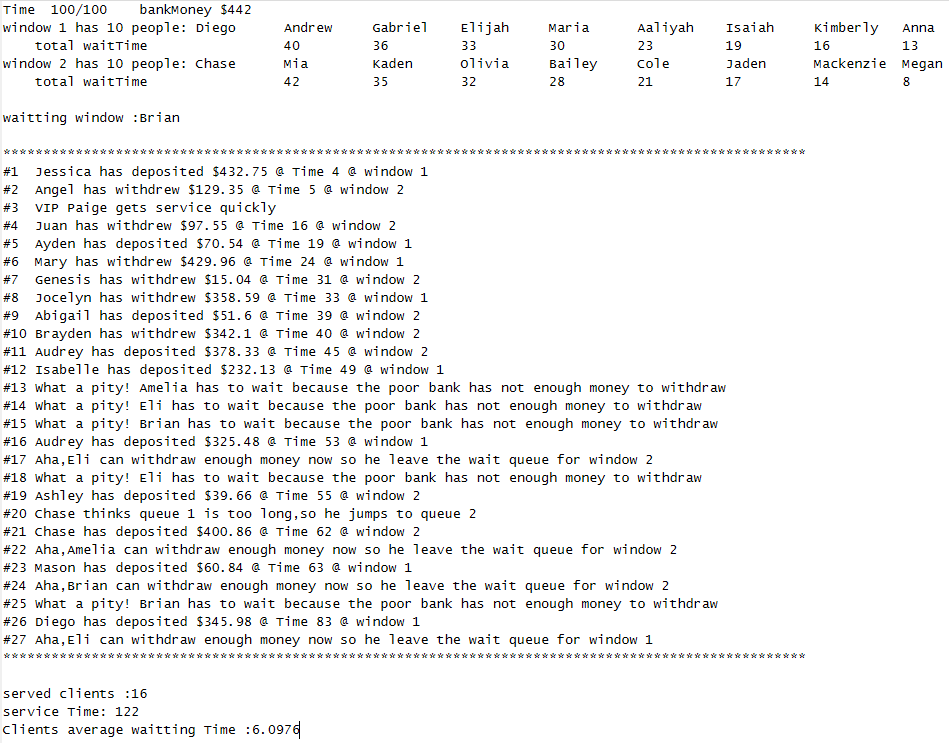
\includegraphics[width=1\textwidth]{result.png}
\end{figure}
\subsection{输入1000,50,30,80,4}
\begin{figure}[H]
  \centering
  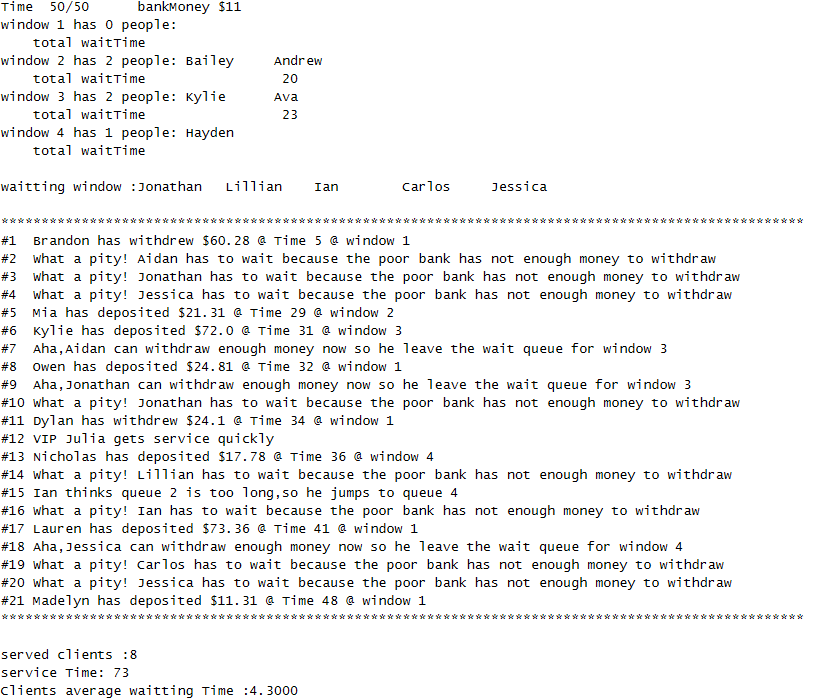
\includegraphics[width=1\textwidth]{result2.png}
\end{figure}
\subsection{输入50000,60,40,300,6}
\begin{figure}[H]
  \centering
  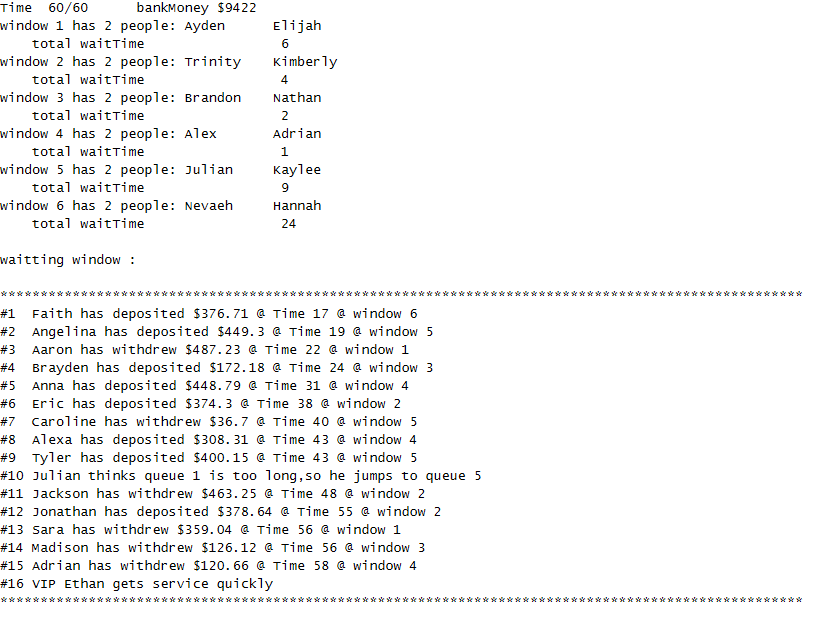
\includegraphics[width=1\textwidth]{result3.png}
\end{figure}
\section{附录}
源文件
bankSimulate.py
\end{document}